\section{Experiment Methodology}
\label{sec:experimentmethodology}

We start with a description of our system setup, including an overview of the components of our sniffer devices. We then present details about the two testbeds where we conducted our experiments. Finally, we round up this section by discussing the data collection process.

\subsection{System Setup}
\label{subsec:systemsetup}

As mentioned briefly in Section \ref{sec:introduction}, WiGEM uses an infrastructure based
architecture. The system has two main components: stationary sniffer devices in the target space and a centralized server running the WiGEM algorithm. Sniffers provide overlapping coverage of the target area (similar to WLAN APs). The server notifies the sniffers about the MAC id of the target device, the channel number and the listening period. The sniffers then record the RSSI of all packets received that match the server's query. The recorded information is sent to the server which then makes a location estimation using the WiGEM algorithm.

In the current prototype, the server communicates with the sniffer devices using in-building power-line network. In the ultimate embodiment, the sniffer functionality could be integrated directly into the WLAN APs. If necessary and appropriate, a localization application can also run on the client that downloads the building map as soon as it gets connected to the WLAN, sends a localization request to the WLAN and shows the location on the map. 

\subsubsection{Sniffer Information}
\label{subsec:snifferinformation}

%The sniffer devices are responsible for capturing wireless transmissions made by a Tx-client. 

We use Soekris net4801~\cite{soekris}  SBCs as sniffer
devices with atheros-based CM9 cards for wireless captures. The sniffers run Pyramid Linux (version 2.6.16-metrix). The default
MadWiFi driver is used comes with this distribution (0.9.4.5:svn 1485). 

To capture packets the standard Tcpdump tool (version 4.0.0/libpcap version 0.9.8) is used. To obtain signal strength information, the MadWiFi driver allows a
monitor mode interface to be created and configured with the radio tap header support. 
The radio tap header reports the SNR (in dB) as the RSSI. This is what we use directly. 
Since the noise floor reported by the cards is constant (-95dBm), the RSSI value 
is also the same as the RSS (in dBm) with a constant difference. 

%ra header we can extract the
%RSSI of each packet received by the sniffer. We verified that the MadWifi driver had a fixed noise-floor in each of our
%cm9 cards (-95 dbm). In fact the received signal strength of a frame reported by the MadWiFi driver is actually the SNR value (in db) obtained after subtracting the noise-floor from the raw signal strength value. We work directly with the RSSI value (in db) as reported by the driver.

\begin{figure*}
	\centering
		\subfloat[CEWIT testbed]{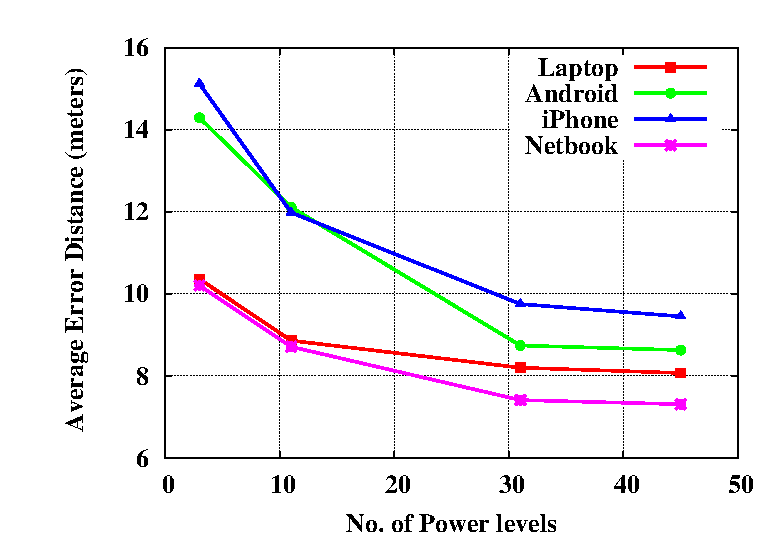
\includegraphics[height=1.5in, width=2.5in]{Figs4Paper/CEWIT/PowerPlot4Paper_CEWIT/PwrLvlPlot_cewit.eps}}
		\subfloat[CSD testbed]{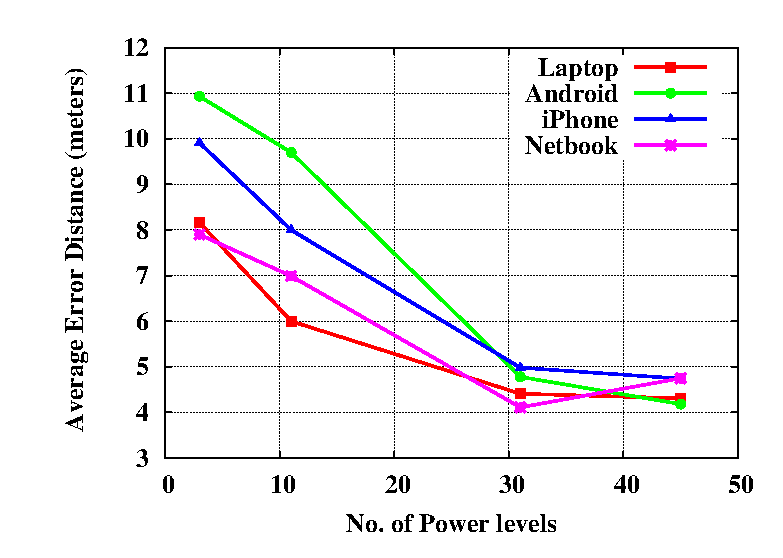
\includegraphics[height=1.5in, width=2.5in]{Figs4Paper/CSD/PowerPlot4Paper_CSD/PwrLvlPlot_csd.eps}}
	\caption{Average error distance results for WiGEM
	as a function of the number of power levels.}
	\label{fig:powerlevelsvserrordistance}
\end{figure*}

\subsection{Testbed Details}
\label{subsec:testbeddetails}

Two different indoor testbeds are used for validation. The first building, henceforth called CEWIT, is a research and development center at Stony Brook University with a dimension of 65 meter $\times$ 50  meter. The L-shaped floor comprises of several obstructions in the form of walls of various types, glass and metal doors, office furnitures, server-rack cabinets etc. The second, building henceforth called CSD, is part of the building housing the computer science department. See Figure~\ref{fig:experimenttestbed}. This rectangular-shaped floor has a dimension of 20 meter $\times$ 30 meter and also have walls and various partitions and office furnitures. Both these testbeds had a continuous flux of people moving around in the building at the time
the experiments were conducted. The CEWIT and CSD testbeds use 6 and 4 sniffers respectively. 
See Figure~\ref{fig:experimenttestbed} for the sniffer locations. 

\subsection{Data Collection Methodology}
\label{subsec:datacollectionmethodology}

The CEWIT testbed is discretized into 45 distinct locations roughly every 5.5 meters. The CSD testbed is divided into 27 distinct locations roughly every 3.3 meters. See Figure~\ref{fig:experimenttestbed}. Multiple device types are used. For each device, we transmit 200 ping packets from every distinct location of the corresponding testbed. This is typically accomplished by having 
the user hold the mobile device and walk across the floor of the building briefly stopping at each marked location to transmit 200 ping packets. The ground truth is noted at each location before moving on to the new location. Note that the ground truth information is used only for evaluation of the localization error and is not supplied to WiGEM for training. Each ping packet is separated uniformly apart at a rate of 1 per second. On the server, the sequence number in the ping packet is used to form the vector of RSSI values recorded by individual sniffers for each transmission. Thus, from each distinct location on the map and for each device type, we have a set of 200 RSSI tuples. This comprises our entire data set that we use in this paper. Experiments on RADAR and Probabilistic (described later in this paper) use a subset of this dataset for building the RF signal map and the remainder data for calculating localization error. 

\subsubsection{Test Devices}
\label{subsubsec:testdevices}

Four different wireless devices are used - a laptop, an android phone, an iphone and a netbook. The laptop is a Dell Inspiron 1545 running Ubuntu v9.04. The android phone is a Google Nexus One. An iphone 3GS (iOS version 4.2.1) is also used. The netbook used is a Dell Latitude 2110 running Ubuntu v9.10. Each device is using its default driver and default power levels for WiFi transmissions. %The devices are henceforth referred to as {\it Laptop}, {\it Android}, {\it iPhone} and {\it Netbook} respectively. 
The data is collected over a span of several days. The devices are not oriented
in any specific direction while making the ping transmissions. The orientation is simply left to the user's choice or convenience. 

%\subsubsection{Sniffer Position}
%\label{subsubsec:snifferposition}
%
%The CEWIT and CSD testbeds have six and four sniffers respectively. See Figure \ref{fig:experimenttestbed}. We assume knowledge of the sniffer positions in the map and use this information to calculate the signal strength values given by the indoor radio propagation model (Equation \ref{eqn:pathloss_2}). These values are used to initialize our algorithm as explained in Section \ref{subsec:handlingidentifiabilityinourmodel} .
